% Copied from:
% http://mirror.its.dal.ca/ctan/macros/latex/contrib/IEEEtran/bare_conf.tex
\documentclass[conference]{IEEEtran}
% Some Computer Society conferences also require the compsoc mode option,
% but others use the standard conference format.
%
% If IEEEtran.cls has not been installed into the LaTeX system files,
% manually specify the path to it like:
% \documentclass[conference]{../sty/IEEEtran}

\usepackage[utf8]{inputenc}
\usepackage{enumitem}
\setlist[description]{leftmargin=1cm,labelindent=\parindent}

\usepackage{balance}
\usepackage{changepage}
\usepackage[hyphenbreaks]{breakurl}
\def\UrlBreaks{\do\/\do-}

% For source code listings.
\usepackage{listings}
\lstset{language=Java}

% For the Hassanbox
\usepackage{framed}

% For colours
\usepackage{xcolor}
\definecolor{additionscol}{HTML}{72E0E0}
\definecolor{deletionscol}{HTML}{BB4466}

\newcommand\crule[3][black]{\textcolor{#1}{\rule{#2}{#3}}}

\newcommand\additionsbox[1]{\crule[additionscol]{#1}{#1}}
\newcommand\deletionsbox[1]{\crule[deletionscol]{#1}{#1}}



% Some very useful LaTeX packages include:
% (uncomment the ones you want to load)


% *** MISC UTILITY PACKAGES ***
%
%\usepackage{ifpdf}
% Heiko Oberdiek's ifpdf.sty is very useful if you need conditional
% compilation based on whether the output is pdf or dvi.
% usage:
% \ifpdf
%   % pdf code
% \else
%   % dvi code
% \fi
% The latest version of ifpdf.sty can be obtained from:
% http://www.ctan.org/pkg/ifpdf
% Also, note that IEEEtran.cls V1.7 and later provides a builtin
% \ifCLASSINFOpdf conditional that works the same way.
% When switching from latex to pdflatex and vice-versa, the compiler may
% have to be run twice to clear warning/error messages.






% *** CITATION PACKAGES ***
%
%\usepackage{cite}
% cite.sty was written by Donald Arseneau
% V1.6 and later of IEEEtran pre-defines the format of the cite.sty package
% \cite{} output to follow that of the IEEE. Loading the cite package will
% result in citation numbers being automatically sorted and properly
% "compressed/ranged". e.g., [1], [9], [2], [7], [5], [6] without using
% cite.sty will become [1], [2], [5]--[7], [9] using cite.sty. cite.sty's
% \cite will automatically add leading space, if needed. Use cite.sty's
% noadjust option (cite.sty V3.8 and later) if you want to turn this off
% such as if a citation ever needs to be enclosed in parenthesis.
% cite.sty is already installed on most LaTeX systems. Be sure and use
% version 5.0 (2009-03-20) and later if using hyperref.sty.
% The latest version can be obtained at:
% http://www.ctan.org/pkg/cite
% The documentation is contained in the cite.sty file itself.






% *** GRAPHICS RELATED PACKAGES ***
%
\ifCLASSINFOpdf
  \usepackage[pdftex]{graphicx}
  \usepackage{epstopdf}
  % declare the path(s) where your graphic files are
 \graphicspath{{diagrams/}}
  % and their extensions so you won't have to specify these with
  % every instance of \includegraphics
  \DeclareGraphicsExtensions{.pdf,.jpeg,.png,.eps}
\else
  \GenericError{}
  {This document will not compile on DVI devices!}
  {It contains images unsupported by DVI (namely, PNG images).}
  {}

  % or other class option (dvipsone, dvipdf, if not using dvips). graphicx
  % will default to the driver specified in the system graphics.cfg if no
  % driver is specified.
  \usepackage[dvips]{graphicx}
  % declare the path(s) where your graphic files are
  \graphicspath{{diagrams/}}
  % and their extensions so you won't have to specify these with
  % every instance of \includegraphics
  \DeclareGraphicsExtensions{.eps}
\fi
% graphicx was written by David Carlisle and Sebastian Rahtz. It is
% required if you want graphics, photos, etc. graphicx.sty is already
% installed on most LaTeX systems. The latest version and documentation
% can be obtained at:
% http://www.ctan.org/pkg/graphicx
% Another good source of documentation is "Using Imported Graphics in
% LaTeX2e" by Keith Reckdahl which can be found at:
% http://www.ctan.org/pkg/epslatex
%
% latex, and pdflatex in dvi mode, support graphics in encapsulated
% postscript (.eps) format. pdflatex in pdf mode supports graphics
% in .pdf, .jpeg, .png and .mps (metapost) formats. Users should ensure
% that all non-photo figures use a vector format (.eps, .pdf, .mps) and
% not a bitmapped formats (.jpeg, .png). The IEEE frowns on bitmapped formats
% which can result in "jaggedy"/blurry rendering of lines and letters as
% well as large increases in file sizes.
%
% You can find documentation about the pdfTeX application at:
% http://www.tug.org/applications/pdftex





% *** MATH PACKAGES ***
%
%\usepackage{amsmath}
% A popular package from the American Mathematical Society that provides
% many useful and powerful commands for dealing with mathematics.
%
% Note that the amsmath package sets \interdisplaylinepenalty to 10000
% thus preventing page breaks from occurring within multiline equations. Use:
%\interdisplaylinepenalty=2500
% after loading amsmath to restore such page breaks as IEEEtran.cls normally
% does. amsmath.sty is already installed on most LaTeX systems. The latest
% version and documentation can be obtained at:
% http://www.ctan.org/pkg/amsmath





% *** SPECIALIZED LIST PACKAGES ***
%
%\usepackage{algorithmic}
% algorithmic.sty was written by Peter Williams and Rogerio Brito.
% This package provides an algorithmic environment fo describing algorithms.
% You can use the algorithmic environment in-text or within a figure
% environment to provide for a floating algorithm. Do NOT use the algorithm
% floating environment provided by algorithm.sty (by the same authors) or
% algorithm2e.sty (by Christophe Fiorio) as the IEEE does not use dedicated
% algorithm float types and packages that provide these will not provide
% correct IEEE style captions. The latest version and documentation of
% algorithmic.sty can be obtained at:
% http://www.ctan.org/pkg/algorithms
% Also of interest may be the (relatively newer and more customizable)
% algorithmicx.sty package by Szasz Janos:
% http://www.ctan.org/pkg/algorithmicx




% *** ALIGNMENT PACKAGES ***
%
%\usepackage{array}
% Frank Mittelbach's and David Carlisle's array.sty patches and improves
% the standard LaTeX2e array and tabular environments to provide better
% appearance and additional user controls. As the default LaTeX2e table
% generation code is lacking to the point of almost being broken with
% respect to the quality of the end results, all users are strongly
% advised to use an enhanced (at the very least that provided by array.sty)
% set of table tools. array.sty is already installed on most systems. The
% latest version and documentation can be obtained at:
% http://www.ctan.org/pkg/array


% IEEEtran contains the IEEEeqnarray family of commands that can be used to
% generate multiline equations as well as matrices, tables, etc., of high
% quality.




% *** SUBFIGURE PACKAGES ***
%\ifCLASSOPTIONcompsoc
%  \usepackage[caption=false,font=normalsize,labelfont=sf,textfont=sf]{subfig}
%\else
%  \usepackage[caption=false,font=footnotesize]{subfig}
%\fi
% subfig.sty, written by Steven Douglas Cochran, is the modern replacement
% for subfigure.sty, the latter of which is no longer maintained and is
% incompatible with some LaTeX packages including fixltx2e. However,
% subfig.sty requires and automatically loads Axel Sommerfeldt's caption.sty
% which will override IEEEtran.cls' handling of captions and this will result
% in non-IEEE style figure/table captions. To prevent this problem, be sure
% and invoke subfig.sty's "caption=false" package option (available since
% subfig.sty version 1.3, 2005/06/28) as this is will preserve IEEEtran.cls
% handling of captions.
% Note that the Computer Society format requires a larger sans serif font
% than the serif footnote size font used in traditional IEEE formatting
% and thus the need to invoke different subfig.sty package options depending
% on whether compsoc mode has been enabled.
%
% The latest version and documentation of subfig.sty can be obtained at:
% http://www.ctan.org/pkg/subfig




% *** FLOAT PACKAGES ***
%
%\usepackage{fixltx2e}
% fixltx2e, the successor to the earlier fix2col.sty, was written by
% Frank Mittelbach and David Carlisle. This package corrects a few problems
% in the LaTeX2e kernel, the most notable of which is that in current
% LaTeX2e releases, the ordering of single and double column floats is not
% guaranteed to be preserved. Thus, an unpatched LaTeX2e can allow a
% single column figure to be placed prior to an earlier double column
% figure.
% Be aware that LaTeX2e kernels dated 2015 and later have fixltx2e.sty's
% corrections already built into the system in which case a warning will
% be issued if an attempt is made to load fixltx2e.sty as it is no longer
% needed.
% The latest version and documentation can be found at:
% http://www.ctan.org/pkg/fixltx2e


%\usepackage{stfloats}
% stfloats.sty was written by Sigitas Tolusis. This package gives LaTeX2e
% the ability to do double column floats at the bottom of the page as well
% as the top. (e.g., "\begin{figure*}[!b]" is not normally possible in
% LaTeX2e). It also provides a command:
%\fnbelowfloat
% to enable the placement of footnotes below bottom floats (the standard
% LaTeX2e kernel puts them above bottom floats). This is an invasive package
% which rewrites many portions of the LaTeX2e float routines. It may not work
% with other packages that modify the LaTeX2e float routines. The latest
% version and documentation can be obtained at:
% http://www.ctan.org/pkg/stfloats
% Do not use the stfloats baselinefloat ability as the IEEE does not allow
% \baselineskip to stretch. Authors submitting work to the IEEE should note
% that the IEEE rarely uses double column equations and that authors should try
% to avoid such use. Do not be tempted to use the cuted.sty or midfloat.sty
% packages (also by Sigitas Tolusis) as the IEEE does not format its papers in
% such ways.
% Do not attempt to use stfloats with fixltx2e as they are incompatible.
% Instead, use Morten Hogholm'a dblfloatfix which combines the features
% of both fixltx2e and stfloats:
%
% \usepackage{dblfloatfix}
% The latest version can be found at:
% http://www.ctan.org/pkg/dblfloatfix




% *** PDF, URL AND HYPERLINK PACKAGES ***

\usepackage{url}
% url.sty was written by Donald Arseneau. It provides better support for
% handling and breaking URLs. url.sty is already installed on most LaTeX
% systems. The latest version and documentation can be obtained at:
% http://www.ctan.org/pkg/url
% Basically, \url{my_url_here}.




% *** Do not adjust lengths that control margins, column widths, etc. ***
% *** Do not use packages that alter fonts (such as pslatex).         ***
% There should be no need to do such things with IEEEtran.cls V1.6 and later.
% (Unless specifically asked to do so by the journal or conference you plan
% to submit to, of course. )


% correct bad hyphenation here
\hyphenation{op-tical net-works semi-conduc-tor}


\begin{document}
%
% paper title
% Titles are generally capitalized except for words such as a, an, and, as,
% at, but, by, for, in, nor, of, on, or, the, to and up, which are usually
% not capitalized unless they are the first or last word of the title.
% Linebreaks \\ can be used within to get better formatting as desired.
% Do not put math or special symbols in the title.
\title{Visualizing Project Evolution Through Abstract Syntax Tree Analysis}


% author names and affiliations
% use a multiple column layout for up to three different
% affiliations
%\author{\IEEEauthorblockN{Michael D. Feist \and Eddie Antonio Santos \and
%  Ian Watts \and Abram Hindle}
%\IEEEauthorblockA{Department of Computing Science\\
%University of Alberta\\
%Edmonton, Canada\\
%\{mdfeist,easantos,watts1,hindle1\}@ualberta.ca}}

% conference papers do not typically use \thanks and this command
% is locked out in conference mode. If really needed, such as for
% the acknowledgment of grants, issue a \IEEEoverridecommandlockouts
% after \documentclass

% for over three affiliations, or if they all won't fit within the width
% of the page, use this alternative format:
%
\author{\IEEEauthorblockN{Michael D. Feist,
Eddie Antonio Santos,
Ian Watts,
Abram Hindle}
\IEEEauthorblockA{Department of Computing Science\\
University of Alberta\\
Edmonton, Canada\\
\{mdfeist,easantos,watts1,hindle1\}@ualberta.ca}}

% use for special paper notices
%\IEEEspecialpapernotice{(Invited Paper)}

% make the title area
\maketitle


% Copyright (C) 2016 Michael D. Feist, Eddie Antonio Santos, Ian Watts, Abram Hindle
% 
% All TeX sources are licensed under Creative Commons Attribution-NoDerivatives 4.0 International (CC BY-ND 4.0) license.
% See terms at <http://creativecommons.org/licenses/by-nd/4.0/>

% === above this line ===
% preamble
% begin document
% maketitle

\begin{abstract}
What is a developer's contribution to a repository? By only counting commits and number of lines changed, existing tools that visualize source code repositories (such as GitHub's graphs) fall short on showing the effective contributions made by each developer. When many commits are viewed as a group, the details are lost. Commit information can be misleading since lines of code give no indication of what was actually being worked on without careful examination of the changed code. Providing a semantic view of this information could provide deeper insights into how software projects evolve since changes to design and features are not clearly visible from line changes alone. We present TypeV: a method for visualizing Java source code repositories. Instead of counting line changes in a commit we extract detailed type information over time by using the differences between abstract syntax trees (ASTs). We are then able to track the additions and deletions of declarations and invocations for each type. Furthermore, we can track each author's type usage over time. Using TypeV, we examine specific cases in well-known repositories where our tool reveals interesting and useful information. We then compare type coverage information from the AST compared to file coverage to determine if unique information is provided by type information.
\end{abstract}

% no keywords

\IEEEpeerreviewmaketitle%

\begin{figure*}[t]
\centering
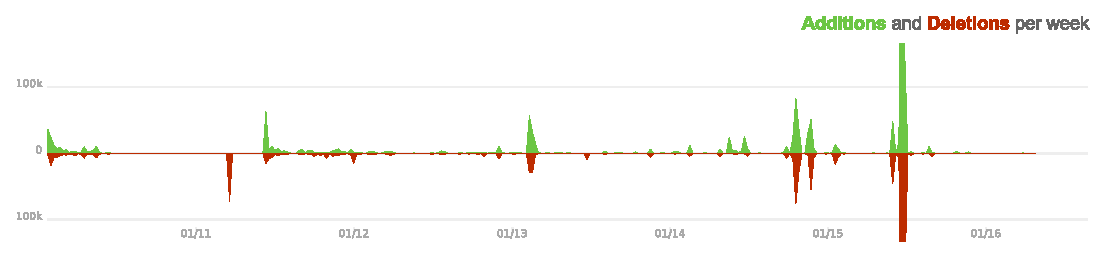
\includegraphics[width=\textwidth]{antlr4-code-freq}
\caption{GitHub's code frequency graph for ANTLR4. Note that the graph was cropped to better show the details. Thus, the changes that occur in mid 2015 are much larger than shown. The additions reach over 400k and the deletions are over 300k.}
\label{fig:GH_code_freq}
\end{figure*}

\section{Introduction}

Source code is often represented as text in a source code file. This text is then parsed by a compiler or interpreter with the intent of eventually executing the code represented by the source text. While programmers may type in individual characters, their intention is at a much higher level. Their intent is written in tokens that represent statements, identifiers, and types that are used to solve their problems. Programmers solve problems in a way that is readable to other developers and executable by a computer. The programmer rarely operates at the character level, or even the line level, so why should our visualizations of source code operate at granularities unfamiliar to developers?

The plain text nature of software does not stop at the source code level. The history and evolution of a software project is often tracked by version control systems, such as Git, in a programming language agnostic way. Updates to source code, documentation, and tests are recorded in the form of commits, which store the differences in lines of text in a file between each subsequent revision of the software. Version control systems become vital for large projects since individual changes would be impossible to track manually. Large projects have thousands of individual changes made by many different developers. With more changes to peruse, it becomes more difficult to see how a project is evolving over time since there is so much information to look through. Hosting services for Git repositories often provide some basic tools for analyzing projects over time~\cite{github-graphs,bitbucket-graphs}; however, as we will show, these tools often lack the kind of detail to gather insightful analysis. As with source code, commits operate at the text level. While commits may store individual changes as lines of code, they imply a change in the \emph{structure} of software.  By visualizing lines changed, or files changed, many current tools for software projects rarely capture the \emph{meaning} behind each commit; lines of code alone do not describe how a repository changed at a particular point in time. Thus, information regarding contributions from developers is often misleading since the number of commits and lines of code changed do not necessarily reflect meaningful changes to a code repository~\cite{robles2014}. In this paper, we will show that abstract syntax trees (ASTs) can be used to create \emph{semantically-aware} software evolution visualizations.

Consider GitHub graphs~\cite{github-graphs}: visualizations that are easily available to software developers using GitHub to host their Git software repositories. GitHub's graphs use line and commit information exclusively. In the case of the ANTLR4 project (Figure~\ref{fig:GH_code_freq}), this code frequency chart creates more questions than it answers. What happened at those big spikes of line changes in the graph? One of the spikes is so large, we had to crop the image in order to show the magnitude of the other changes. How did these large changes affect the code base? Who committed these large changes? Was it a team of contributors or one particularly prolific programmer? Plotting the number of lines changed may be misleading. A huge spike in additions may be caused by a number of reasons, such as the inclusion of automatically-generated documentation, the inclusion of an external library, or perhaps a massive refactoring effort~\cite{Hindle:2008:LCT:1370750.1370773}.

The goal of a software evolution visualization is to provide an alternate view that provides insight into the development of the software that is otherwise unavailable. By visualizing changes to lines and files, one is tracking the changes in text---not software. Instead, we promote \emph{semantically-aware visualizations} that visualize the structural changes in code. In our case these are changes in variable declarations, invocations of methods, and usage of types. Others have explored semantically-aware visualization~\cite{sourcevis,6980224,Kim:2009:DRS:1555001.1555046,7332410}, however, we show that this can be done with ASTs.

In this paper, we propose a semantically-aware visualization method that tracks the changes in type usage and method invocations over time. Using commits, we are able to keep track of \emph{who} is using what types. We then present this data using time-proven visualizations. We claim that type usage and method invocation offers more insight than line-based, file-based, and commit-based methods of visualization and analysis. For simplicity, we analyze only Java projects, as it allowed us to quickly develop and test our software. However, since the approach described in this paper can be generally applied to any statically-typed language, it can be adapted to other programming languages. Our goal is to describe a methodology for obtaining richer, more meaningful data from source code repositories which can be used for more insightful analyses.

In the following sections of the paper we will describe our tool, TypeV, that we developed to compute and visualize changes to types by author used in a project over time. TypeV is able to extract type information from a repository by computing commit-by-commit abstract syntax tree differences, which we describe in Section~\ref{sec:methodology}. In this paper, we answer the following questions: \\ \\
\textbf{RQ1:} How can we extract type and method usage from repositories over time? \\ \\
\textbf{RQ2:} How does type coverage compare to file coverage?
\\ \\
\textbf{RQ3:} Does the type information give any interesting or useful insight into the project?

\section{Related Work}

We examined research which analyses software repositories for information on language and feature usage, tools for visualizing project evolution, collaboration in software repositories and other tools for understanding repositories.

\subsection{Analysis of Languages and Features}

Analyzing source code is a popular research topic and Java is often chosen as the subject of study due to its popularity and abundance of tools. Grechanik \textit{et al.}~\cite{Grechanik:2010:EIL:1852786.1852801} examined the structure of Java programs mined from 2080 programs. This paper examined the breakdown of syntactic structures in open source repositories, however it does not consider per author statistics. Parnin \textit{et al.}~\cite{Parnin:2011:JGA:1985441.1985446} mined repositories to see how Java generics have been used in open source projects and found that generic usages were often introduced by a single developer in a project and were primarily being used for collecting and traversing lists of objects.

Further analysis of the Java language has been done using ASTs. L\"{a}mmel \textit{et al.}~\cite{Lammel:2011:LAA:1982185.1982471} used ASTs to examine the usage of APIs in Java projects. They found which APIs are popular and if they were used in a framework-like manner. Dyer \textit{et al.}~\cite{Dyer:2014:MBA:2568225.2568295} mined AST nodes to study the use of new Java language features over time. The authors found the most popular features and the adoption rate of new features over time. They did not check to see how much a developer used a feature but instead checked to see if they used it at all. In a more general analysis of programming languages, Meyerovich and Rabkin \cite{Meyerovich:2013:EAP:2509136.2509515} surveyed developers and examined repositories to learn about language adoption and usage. Developers feel that certain language features are more important than others.

The focus of these papers was on how programming languages and features are used by looking at many repositories. Java is a statically-typed language---its types are checked at compile time---yet there is no focus specifically on how types are used throughout a project. Type data may provide additional information on how developers use languages but this has yet to be explored.

\subsection{Visualizing Project Evolution}

Several visualizations tools have been created to understand how a software system changes over time. Wu \textit{et al.}~\cite{wu2004a} explored punctuated changes of software repositories with a tool that generates an Evolution Spectrograph. In this visualization, each file has a row in the chart and each cell represents a section of time where an incoming or outgoing dependency can be changed. The colour is determined by the frequency of change. This work was continued to show file directories and display the cardinality of a developer's commits in Wu \textit{et al.}~\cite{wu2004}. The cardinality of a commit is the number of files or subsystems it affects in a system, indicating the scope of the change. Other tools also look at changes in code dependencies~\cite{6980224} or files~\cite{6650525, 7332421, voinea2006} over time. Alcocer \textit{et al.}~\cite{6650523} create a Performance Evolution Blueprint, which displays the changes in performance over time as a project evolves. Ogawa and Ma created code\_swarm~\cite{codeswarm}, a generative art visualization which presents the progressive evolution of file changes made by authors in a source control repository over time. Gource~\cite{gource} is a similar visualization, showing an animated force-directed tree of the file hierarchy as authors make changes to files in the source code repository over time. Ens \textit{et al.} created ChronoTwigger to visualize the co-evolution of source and test files~\cite{6980223}. This allowed testing practices to be more closely examined. Anslow \textit{et al.}~\cite{sourcevis} created SourceVis, a suite of software visualizations including visualizations for semantically-aware project evolution. SourceVis displays the evolution of Java source code metrics such as number of packages, classes, methods, and fields.

Tools also exist which track changes over time in a more complex manner. Kim \textit{et al.}~\cite{Kim:2009:DRS:1555001.1555046} built a tool called Logical Structural Diff (LSdiff) which examines code changes and produces logical rules to represent them. Changes which do not match the rules are then pointed out to the developer. Reiss and Tarvo created an IDE which allows users to see the history of files and changes to lines of code from each author as they are editing a project~\cite{6650521}. Van Hees and Hage use a voronoi treemap to visualize changes in class and method structure~\cite{7332410}. Servant and Jones created CHRONOS, a tool which creates a timeline of changes to a selection of code as well as the ability to query those changes~\cite{6650547}.



\subsection{Project Collaboration}

There is also research on how developers use software repositories to collaborate. Wagstrom \textit{et al.}~\cite{Patrick:Wagstrom:2012} explored the roles that developers take in networked, social development environments like GitHub. These roles were defined by their level of contribution as well as the types of issues they dealt with. They found that developers will take on multiple roles in a project and will sometimes fulfill the same role across different projects. Lee \textit{et al.}~\cite{lee2013} developed a tool for visualizing the branching structure of Git repositories. This was used to analyze concurrent workflows in popular open source repositories. Elsen also created a visualization for branches in Git, with the ability to expand branches to view the directory structure of a project at that point~\cite{6650522}.   Shrestha \textit{et al.} made a visualization for the geographic location of a commit and~\cite{6650532} and Minelli \textit{et al.}~\cite{6980226} looked at the real time changes developers made to a repository.

\subsection{Non-academic works}

Some visualization tools are made for managing or making decisions about software rather than studying the changes taking place in an academic context. EasyBi~\cite{EasyBi} is a service that provides additional visualizations for Git repositories for the purpose of business decisions. EasyBi works by taking the \texttt{git log} file and generating charts and graphs from it. It tries to solve the issue of summarizing many commits and has greater controls for granularity and authors but still operates on commits and line differences. The Gitinspector project~\cite{Gitinspector} is an open source tool for the statistical analysis of Git repositories. It provides an advanced timeline view of changes per author and cumulative statistics but again relies upon the line differences to summarize the work of each author.

Developers using the massively popular GitHub website for hosting their Git repositories instantly have access to basic visualizations, known as GitHub Graphs (Figure~\ref{fig:GH_code_freq})~\cite{github-graphs}. GitHub Graphs tracks contributions based only on the number of commits and number of lines changed. This has the advantage of not relying on the code which was committed. It does not matter what language is used or if errors exist in the commit---GitHub will simply output the number of line additions and deletions. The issue with this type of analysis is that it does not give a clear idea of what is being changed, only that changes have occurred. This data may be lacking, or even misleading which contributes to the need for better tools.

Of the services we have surveyed, none of the tools that visualize project evolution address semantic history extraction using granular type analysis per author via commit-by-commit abstract syntax tree differencing.

\section{Data Extraction}
\label{sec:methodology}

\begin{figure}[!h]
\centering
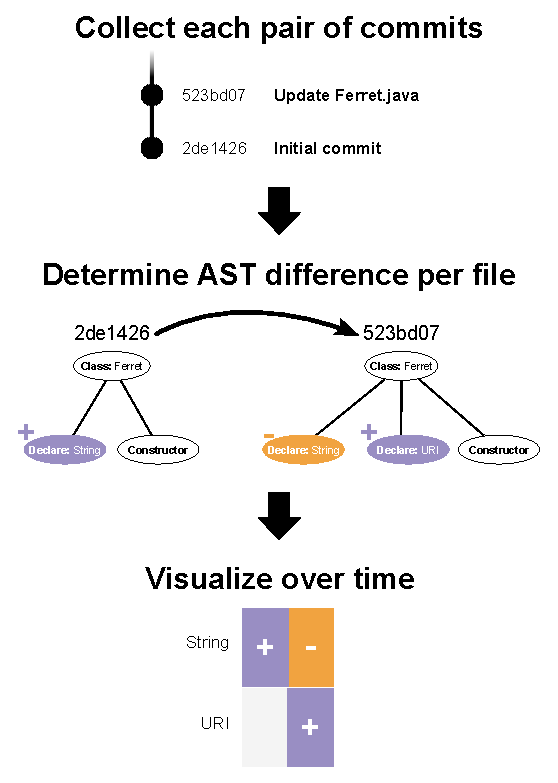
\includegraphics[width=\columnwidth]{context}
\caption{Data extraction pipeline for TypeV. First, we list the commits in branch chronological order. Then we calculate the AST difference between each changed file across each pair of consecutive commits. Finally, we may visualize the information in a variety of ways.}
\label{fig:context}
\end{figure}

Given a Git repository, we want to extract per-author use of types over time. We accomplish this by computing the differences between abstract syntax trees of every consecutive pair of commits (Figure~\ref{fig:context}). This extracted data can then be used in a variety of visualizations as discussed in Section~\ref{sec:viz}. The reason for using ASTs is that they capture the semantics of the code far better than simple line counts.

An \emph{abstract syntax tree} (AST) is a data structure derived from source code that breaks its syntactic constructs into a tree. Each node in the tree represents a syntactically valid chunk of code. This captures the structure of the code in an abstract and tractable manner. When a programmer makes a non-trivial change to a source code file, that difference will be reflected in the AST\@. Non-trivial changes are those that affect how a compiler will interpret the source code, and may have effects on the executable code. Trivial changes are those that have no effect on how a compiler will interpret the source text, such as changing insignificant whitespace or comments in source code. Thus, ASTs of consecutive revisions in a code repository can be compared to see what \emph{structures} a programmer is modifying.

The Java ASTs in our analysis were generated using Spoon~\cite{pawlak:hal-01169705}. Spoon is a tool for transforming and analyzing Java source code. It breaks code up into a meta-model consisting of three parts: structural elements, code elements and references to program elements. According to Spoon's authors: ``The structural part contains the declarations of the program elements, such as interface, class, variable, method, annotation, and enum declarations.  The code part contains the executable Java code, such as the one found in method bodies. The reference part models the references to program elements (for instance a reference to a type)''~\cite{pawlak:hal-01169705}. The Spoon model is convenient because it provides the infrastructure for performing AST differencing (described later) while retaining code elements for analysis afterwards. Spoon also preserves all type and package (library) information, information vital to our semantic analysis.

To determine what has changed between two subsequent commits, we computed their \emph{AST difference}. Given two ASTs, an AST difference (or simply as \emph{AST diff}) states which nodes must be added and which nodes must be removed to transform one tree to the next (step two in Figure~\ref{fig:context}). This allows us to precisely track changes between two consecutive revisions of the same file. For AST diffing, we used GumTree~\cite{falleri:hal-01054552}, an algorithm made to compute the difference between two ASTs generated by Spoon. For new files and deleted files, it is unnecessary to calculate an AST difference; we simply run Spoon on the files and treated everything as an addition or deletion respectively.

Once we calculate the AST diffs, we were able to traverse through the trees to count the number of added or deleted \emph{declarations} and \emph{invocations} for a given type.

\begin{description}
\item [declaration:]
  Stating that use of a field or variable of a given type. For example declaration of a \texttt{String} type variable might look as follows:
  \\
  \begin{adjustwidth}{2.5em}{0pt}
  \texttt{String myString;} \\
  \end{adjustwidth}
\item [invocation:]
  A call site for a method that belongs to a type. For example an invocation of the trim method of a String type might look as follows:
  \\
  \begin{adjustwidth}{2.5em}{0pt}
  \texttt{myString.trim();} \\
  \end{adjustwidth}
\end{description}

Each change of declaration or invocation is detected and tallied per file per commit. These changes are emitted in an ad hoc file format. For example, the following is the output of a commit that changed two declaration of \texttt{String} variables to \texttt{URI} variables:

\begin{verbatim}
#DECLARE | INSERT | java.net.URI | 2
#DECLARE | DELETE | java.lang.String | 2
\end{verbatim}

This states that two declarations of type \texttt{java.net.URI} were added, and two declarations of type \texttt{java.lang.String} were deleted. Note that TypeV is able to find the fully qualified type names. Thus, the source text may not literally have the characters \texttt{java.net.URI}, but Spoon was able to infer from the import statements in the Java source text that references to ``URI'' resolve to the fully-qualified type name \texttt{java.net.URI}. 

\begin{figure}[h]
\centering
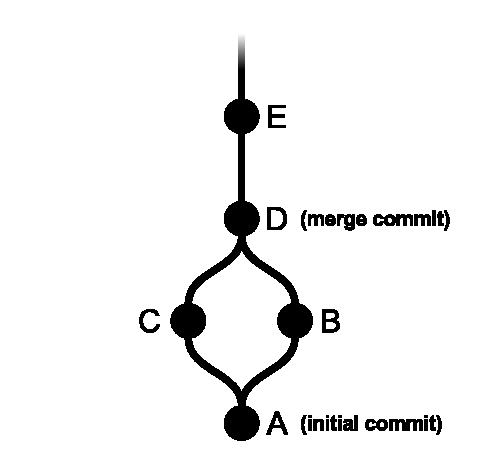
\includegraphics[height=2.5in]{commits_view}
\caption{Commits increase in time from bottom up. Therefore, ASTs from B and C are diff'd against ASTs in A. ASTs from E are diff'd against D. Since D is a merge commit, its changes are ignored as they are recorded in C and B.}
\label{fig:commits}
\end{figure}

In order to gather all the changes for a given repository over time, we generated ASTs for each commit and compared the difference. We did this by running \texttt{git log} over the Git repository and listed all commit IDs in chronological order (Figure~\ref{fig:commits}). For each commit, we collected the following information, as can be seen in Figure~\ref{fig:data-extracted}: the author's name, date of commit, commit ID (SHA), commit message, files the commit edited, and files in the repository at the time of the commit. For all the edited Java files we also compared the file at the time of the commit with its parent commit using AST differencing as described above. We achieved this by invoking \texttt{git difftool} and specifying our AST differencing tool. One case where \texttt{git difftool} fails is when the commit has no parent, such as the initial commit. We were able to handle this by calling \texttt{git show} and saving the output to a temporary file to be used with the AST differencing tool. When calling \texttt{git show} instead of \texttt{git difftool} we treat everything as an addition, as in commit A in Figure~\ref{fig:commits}. Since we compare each commit to its parent as reported by Git, we are able to account for any branching that happened outside the primary branch of the repository (usually named \texttt{master}). If a commit has more than one parent, like commit D in Figure~\ref{fig:commits}, it indicates a merge commit in Git.

We deliberately chose to ignore merge commits. A merge commit has two cases to consider: The first case is when the parents of the commit can be automatically merged. In this case all the relevant changes are already recorded in the parent of the commit so we can safely ignore the merge commit~\cite{git:merge}. The second case occurs when the parents cannot be merged automatically: this is a \emph{merge conflict} which requires manual resolution on the part of a developer. In this case, the developer will try to resolve the issue by modifying code. If we decide to include the merge commit we run into several edge case issues such as how to compare the merge commit with its multiple parent commits and how to account for the possible modifications made to resolve the merge conflict. We could consider comparing the merge commit with only one parent commit at a time; however, we will end up counting all the changes already recorded in the other parent branch. Additionally, all changes made during the resolution of a conflict will be attributed to the author making the merge. This may exclude the author that actually wrote the code in the first place. The other option is to simply ignore the merge commit such that we do not count the changes done during a merge commit. We made the assumptions that merge conflicts occur infrequently and when they do occur, the changes made to resolve a merge conflict are usually minor. Therefore, we chose to ignore merge commits. 

\begin{figure}[h]
\centering
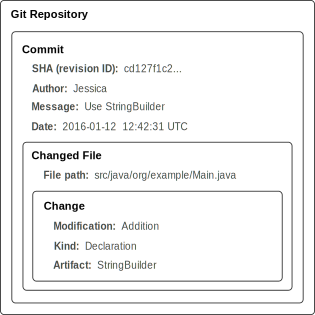
\includegraphics[width=\columnwidth]{data-extracted}
\caption{Hierarchy of data extracted by TypeV. Each repository may have zero or more commits; each commit may have zero or more changed files; each changed files may have zero or more changes, as computed by our AST differencing tool.}
\label{fig:data-extracted}
\end{figure}

The data collected from running the AST differencing component over the commits is saved to a file to be visualized later; this data is in a general format, and is not bound to any particular visualization. Figure~\ref{fig:data-extracted} summarizes the hierarchy of the data extracted by our tool.

The major downside of AST diffs over a method like line count is that ASTs are more expensive to compute. Our experiments were run on a Intel i7 with 16GB of RAM and an SSD. Calculating the AST diffs varied from an hour or two for smaller projects to a couple of days for very large projects. For example ANTLR4 took about 8 hours while Apache BookKeeper only took a couple of hours. The good news for ongoing projects is that AST diffs only need to be computed for new commits; TypeV can resume calculating diffs and augment statistics at any time.

\section{Visualization}

% CITE PAPERS THAT HAVE USED OUR APPROACH!
% AND SAY OUR VISUALIZATIONS ARE EFFECTIVE BY PROXY

% TODO: \cite{sillito2006}

\label{sec:viz}

\begin{figure*}[!ht]
\centering
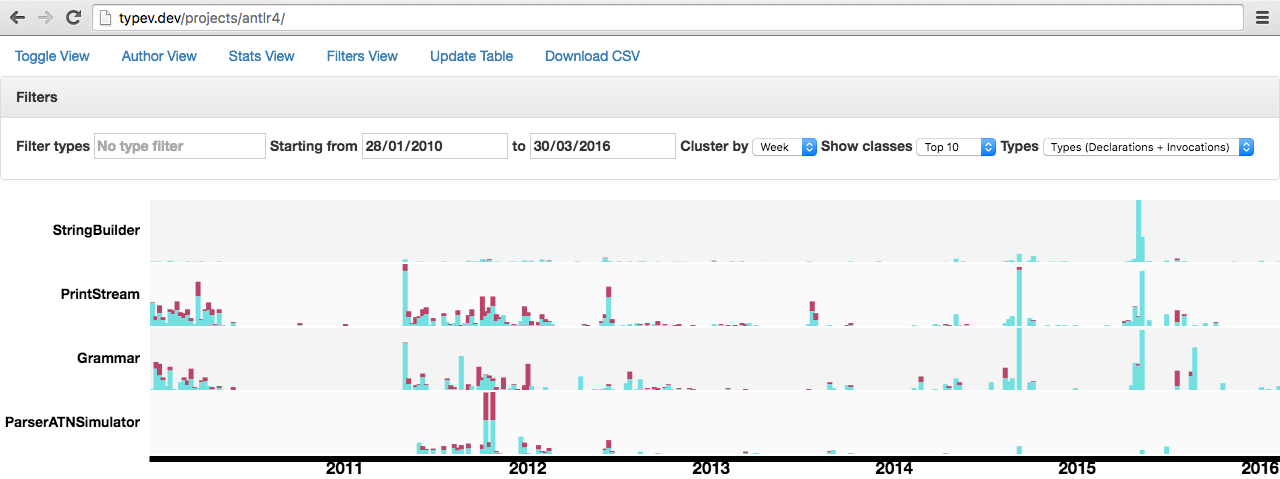
\includegraphics[width=\textwidth]{Screenshot_antlr4}
\caption{Screenshot showing the main view for TypeV. The data being displayed is from the ANTLR4 repository. Light blue bars \additionsbox{10pt} indicate \textbf{additions}; dark red bars \deletionsbox{10pt} indicate \textbf{deletions}.}
\label{fig:main-view}
\end{figure*}

Although rich in detail, the AST diffs are difficult to analyze if displayed in their raw form; hence, we created an HTML5 web visualization application which is intended for developers, project managers, and researchers to use (Figure~\ref{fig:main-view}). The source code for TypeV---both the AST differencing component and the web application---is available online on GitHub.\footnote{\url{https://github.com/mdfeist/TypeV}} A screencast demonstrating its use is also available online.\footnote{\url{https://archive.org/details/typev-demo}}

\subsection{Timeline View}
For our main demonstration of semantically-aware project evolution, we chose an interactive timeline view that displays the most popular types over time. The timeline displays several rows of stacked bar graphs which show changes to an individual type or method over a selectable period of time in a project (Figure~\ref{fig:main-view}). The light blue \additionsbox{10pt} and dark red \deletionsbox{10pt} portions account for the number of additions and deletions respectively, in a similar fashion to GitHub's code frequency graph (Figure~\ref{fig:GH_code_freq}). The height of each bar shows the relative number of changes to a type. The width of each bar is fixed, and represents a time period for binning commits that can be configured to an hour, day, week, or month's worth of commits per each bar. A bar that completely fills its row vertically is the period with the largest number of changes to that type in the visible date range. The height of the other bars in the row are in proportion to the maximum number of changes. The bar height is calculated by multiplying the maximum bar height by the number of changes during that time period divided by the maximum number of changes attested for this type.

One can interact with the overview by hovering and clicking on the bars. When a user mouses over a specific bar in the graph they are given summary information for the type and time period at that location. The information includes the fully-qualified name of the type, the number of commits, the number of authors, the number of additions, the number of deletions, and the start and end date of that time period. If the user clicks on the bar, they are given more detailed statistics which list the authors who made the commits and each commit message. 

To allow for a more detailed analysis of a specific component of the repository we added filtering tools. Users can filter by type name; view changes that fall within a specific start and end date; and select whether to see only declarations of types, types used in declarations and invocations, or only invocations.

One issue with analyzing individual authors is that authors can commit from a variety of different computers which can have different emails and usernames attached to their Git configuration. This may result in one author appearing as several different authors in the \texttt{git log}. There is no perfect way to deal with this problem; however, we added an interface for managing authors. A user can manually specify an author's various aliases using a simple dropdown list. All statistics attributed to an author's various aliases are then remapped as belonging to one canonical author as specified by the user.

In addition, our author managing view also provides a facility for selecting and deselecting authors in the view. Thus, visualization users can focus on the changes made by one author or a group of authors, rather than only having the option of view changes made by all authors cumulatively.

\subsection{Design Decisions}

The purpose of displaying stacked bar charts is that they are a familiar visualization. They can be viewed as an enhanced version of GitHub's code frequency graph~\cite{github-graphs}, with semantic data. We chose to create a similar visualization to GitHub to work with a layout people may already be familiar with and to evaluate our visualization tools' density of data.

The stacked bar graphs succinctly displays the relative amounts of additions and deletions per each time period. This creates a dense view of the project's evolution. We chose to make the height of the bars relative to only the type itself to make it easy for a user to scan a single type and see when it was modified. This makes tasks such as finding a refactoring (Section~\ref{sec:antlr4}) very clear to see simply by browsing the line. We stacked the additions on top of the deletions such that users can immediately compare the relative frequency of changes of a single type throughout the chosen time span.

Our choice of colours was motivated to be high contrast and culturally indicative of their meaning. The particular colours chosen are high contrast, and are distinct to those experiencing protanomaly or deuteranomaly---red-green colour blindness. The red colour suggests a negative valence~\cite{moller2009}, hence suggesting deletions. The blue serves as a contrast to the red, indicating the opposite action (in this case, additions).

The rows are sorted so that the graph for the most used types or methods appear the top and are in descending order of use such that the most frequently used type is the first visible. The height allows users to see when certain types are being edited and ensures that highly used types do not overpower less used types making their changes less significant.

By adding interaction, the user is able to explore the timeline to find the specific information that they are interested in and drill-down at their leisure. Although our tool extracts a great deal of information, users can gradual reveal more information as they need it, rather than be bombarded with all of the information at once.

% TODO: Add design decisions for author merging?

\section{Evaluation}
\label{sec:eval}

% TODO: say all these other tools used file-based stuff:
% gource, github, code_swarm, others...?

\begin{table}[t]
\renewcommand{\arraystretch}{1.3}
\centering
\caption{Summary of projects used in the evaluation.}
\label{tab:project-summary}
\begin{tabular}{c|ccccc}
\hline
\bfseries Project & \bfseries Commits & \bfseries Authors & \bfseries Files &   \bfseries Types &  \bfseries  Changes\\
\hline
ANTLR4 & 3930 & 19 & 1792 & 2635 & 58425\\
BookKeeper & 660 & 10 & 758 & 1872 & 31817\\
Curator & 1524 & 35 & 1211 & 1269 & 27957\\
Tika & 860 & 10 & 604 & 757 & 20764\\
\hline
\multicolumn{6}{p{3.25in}}{\footnotesize Totals for the four projects we analyzed. ``Changes'' refers to the total number of invocation or declaration changes observed from the AST diffs.}
\end{tabular}
\end{table}

\begin{table}[ht]
\renewcommand{\arraystretch}{1.3}
\caption{Comparison of Type Coverage and File Coverage in Projects}
\label{tab:summary}
\centering
\begin{tabular}{c|ccc}
\hline
\bfseries Project & \bfseries Wilcoxon& \bfseries Pearson (linear) & \bfseries Spearman (rank) \\
& $p$-value & Correlation & Correlation \\
\hline
ANTLR4 & $p\ll0.01$ & 0.943 & 0.907\\
BookKeeper & $0.313$ & 0.984 & 0.972\\
Curator & $0.007$ & 0.975 & 0.980\\
Tika & $0.653$ & 0.955 & 0.998\\
\hline
\end{tabular}
\end{table}

\begin{figure}[ht]
\centering
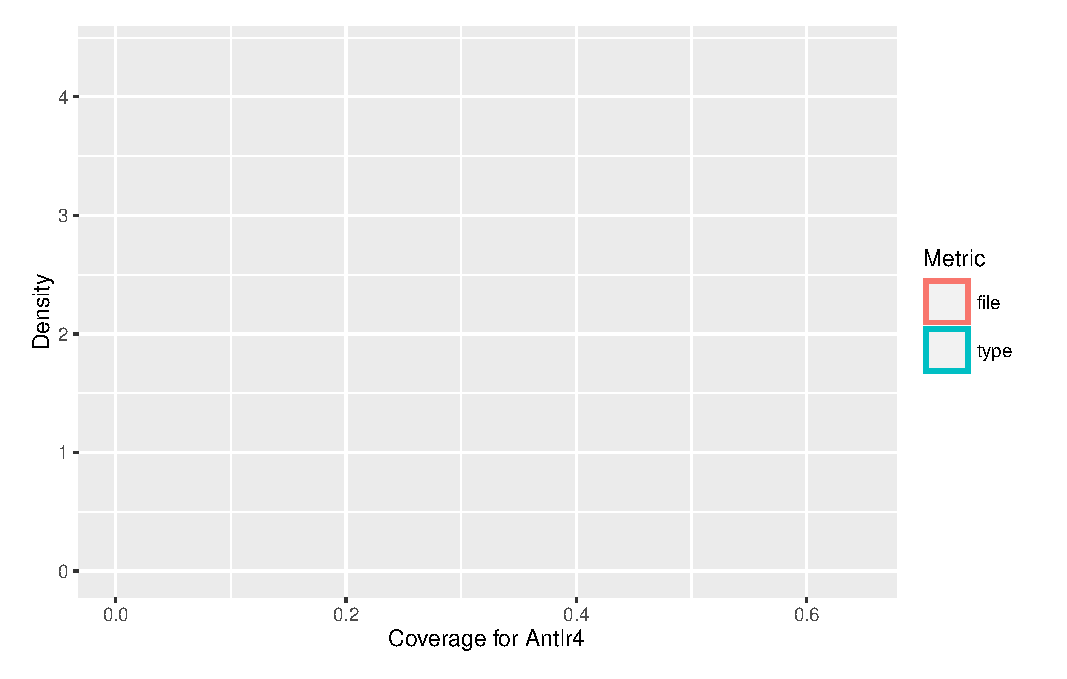
\includegraphics[width=\columnwidth]{antlr-density}
\caption{Density plot of type and file coverage for commits. The graph shows what percentage of type and file coverage the majority of commits have. One can see that the majority of commits have a type and file coverage around 0\% to 20\%. We can also see a difference between these measurements on the higher end of the graph. File coverage seems to have a group of commits that had a file coverage between 20\% and 50\% whereas type coverage have a similar looking grouping but between 40\% and 60\%.\label{fig:antlr4-density}}
\end{figure}

\begin{figure}[ht]
\centering
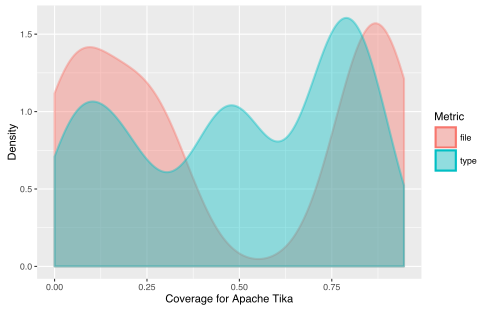
\includegraphics[width=\columnwidth]{tika-density}
\caption{Density of type and file coverage for commits. Here we can see that commits did not have much file coverage between 25\% and 75\%. On the other hand there were a lot of commits that have type coverage around 50\%.\label{fig:tika-density}}
\end{figure}

\textbf{RQ2}: Is it worth the effort of computing commit-by-commit AST differences if we can simply count changes to files? We will answer this question by comparing type coverage and file coverage. We define \emph{type coverage} as the number of types that have been touched out of the total number of types during either a certain time period or the entire project. \emph{File coverage} is the same measurement, but using the number of source files touched instead. File coverage can be trivially determined from an author's commit history. Type coverage, however, is uniquely provided by AST differencing, as we have described.

In Java, a type can be primitive, provided by the language itself, or an object reference. Primitive types are those that are built into the language such as an \texttt{int} or \texttt{char}. Object references point to instances of classes. Java's syntax encourages the creation of classes, thus we expect substantial Java projects to define many domain-specific types. Additionally, Java places the constraint that each source file must define one class. When writing or contributing to a project, the author's choice of which part of the program to edit will in turn affect what types they end up working with --- that is, it will affect the author's type coverage. Similarly, the set of files that an author works with affects that author's file coverage.

To determine if type coverage yields different information than file coverage, we analyzed four open source Java projects: ANTLR4, Apache BookKeeper, Apache Curator and Apache Tika (Figure~\ref{tab:project-summary}). Three of the four projects were collected from the Apache foundation, as they host a large number of well-curated open source Java projects. We counted the file coverage and type coverage on a commit-by-commit basis for each author. That is, each datum represents a commit with three dimensions: file coverage, type coverage, and its commit date. Data is sorted in ascending order of commit date. Table~\ref{tab:summary} lists a summary of the statistics measured.

We displayed the density distributions for two different projects: ANTLR4 (Figure~\ref{fig:antlr4-density}) and Apache Tika (Figure~\ref{fig:tika-density}). These plots show the distribution of the amount of commits that have X\% of type and file coverage. For example, Figure~\ref{fig:tika-density} shows that there are many commits with 50\% type coverage and while there are relatively few commits with 50\% file coverage. This shows that even though the type and file coverage plots may have a similar shape, the commits are showing different levels of information. 

In general, type coverage and file coverage are strongly correlated, both using Pearson (linear) correlation, and Spearman (rank) correlation. As type coverage and file coverage are both cumulative measures, positive correlation is expected. However, even when the distributions are significantly different (as with ANTLR and Curator), the correlation is still strongly positive, but not 100\%. This means that when the coverage for types and files of a commit increase, the relationship is not necessarily one-to-one. This is remarkable in a language like Java, as classes and files are generally in a one-to-one relationship.

We conclude from these findings that type coverage yields related, yet different information than file coverage alone.

\section{Illustrative Case Studies}
\label{sec:cases}

In the following sections, we present case studies demonstrating the extra insight that the AST differencing provides.

\subsection{ANTLR4}\label{sec:antlr4}

\begin{figure}[!ht]
\centering
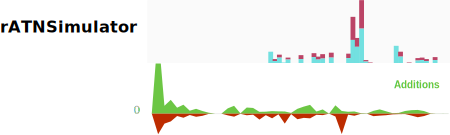
\includegraphics[width=\columnwidth]{ParserATNSimulator-Antlr4-GH-Lines}
\caption{Screenshots of TypeV (above) and GitHub's code frequency graph based on line difference (below). TypeV is showing changes to \texttt{ParserATNSimulator} in ANTLR4 while GitHub's graph is showing all line changes to ANTLR4. The date ranges from approximately April 2011 to April 2012. Note that both the TypeV and GitHub graphs are approximately lined up along the x-axis (time) and that we can see the loss of detail in the GitHub graphs.}
\label{fig:parser}
\end{figure}


We chose ANTLR4 because it is a substantial Java project with a commit history spanning several years. We can also see distinct changes throughout its history.

For example, in December of 2011, in Figure~\ref{fig:parser} we can see that the \texttt{ParserATNSimulator} class has a large amount of additions and deletions in roughly equal proportion. This suggests that \texttt{ParserATNSimulator} is not being removed from the project but instead there is some refactoring being done. If we take a closer look at the commit messages we can see that they mention refactoring and reorganization of code. Zooming in on that date,  shows that during that month they were finishing work on a new version of \texttt{ParserATNSimulator}.

If we tried to do the same analysis with the GitHub tools it would be significantly more difficult to reach this conclusion (Figure~\ref{fig:parser}). First, if we only look at line changes this change to \texttt{ParserATNSimulator} is overwhelmed by other changes and hardly shows up on the GitHub tools. If we did notice an increase in activity we would not know what types were being worked on. Finally, we could not quickly look at the commit messages for that specific time and type if we used the GitHub tools.

Using TypeV we can see that at certain times there were major changes across all types. This shows us when major changes to the code were being done versus code maintenance.

\subsection{Apache BookKeeper}

\begin{figure}[!ht]
\centering

\includegraphics[width=\columnwidth]{bookkeeper_dep}
\caption{Shows deprecated invocation \texttt{getLedgerManagerType()} and replacement invocation \texttt{getLedgerManagerFactoryClass()} for Apache Bookkeeper.}
\label{fig:bookkeeper-depr}
\end{figure}

The purpose of \emph{deprecating} software features is to give developers time to change projects to follow a new or better standard without breaking existing code. When a piece of code becomes deprecated, continuing its use may lead to design flaws or even security vulnerabilities. For example, in Apache Nifi, an earlier version of the software used a compromised key-derivation function; hence, this class was deprecated, but left in for compatibility with older versions of the software~\cite{nifi}. Viewing changes in terms of types can show when usage of deprecated classes are added or removed from a project as well as how many remain over time. Given the time at which a feature was deprecated, seeing the progress of replacement has some important implications. In the case of a security flaw, that time could indicate times at which systems or its users were vulnerable. If a feature is marked for removal, a third party using the deprecated feature has a limited time to make the appropriate changes. Removing all instances of deprecated features could also mean a project can be upgraded to use new tools or features that were not possible when the deprecated features were present.

We searched for Apache foundation projects that featured an instance of deprecation and found Apache BookKeeper. As an Apache Foundation project it is a well-curated example of an open source software project.

Apache Bookkeeper deprecated the method Abstract\-Configuration.\-get\-Ledger\-Manager\-Type() in release 4.2.0\footnote{\url{https://bookkeeper.apache.org/docs/r4.2.0/apidocs/deprecated-list.html}} and replaced it with Abstract\-Configuration.\-get\-Ledger\-Manager\-Factory\-Class(). If we look at get\-Ledger\-Manager\-Type() we can see at the time of the start of the deprecation all instances were removed and get\-Ledger\-Manager\-Factory\-Class() was added (Figure~\ref{fig:bookkeeper-depr}). After the deprecation, we see no more changes to get\-Ledger\-Manager\-Type() and only some additions of get\-Ledger\-Manager\-Factory\-Class().

\section{Discussion}

Having semantically aware evolutionary visualizations also gives users who are unfamiliar with the project at-a-glance information on the evolution of the project.

Having tools for analyzing repositories based on type usage and method invocation benefits many parts of the software development process. Software managers require a high level understanding of the state of a repository and the changes being made which affect the functionality of the software. Tracking developer contributions in a less misleading way is also important for management since important contributions may be small and focused, but nevertheless, significant. Line differences only provide meaningful information when they are analyzed by someone with familiarity with the source code being changed. Providing tools which bring more meaning than line differences would allow people less familiar with the code to understand changes being made. When large changes are made that cover many aspects of a project, it is more useful to see how the change affects the software rather than noting that several thousands of lines have changed. Seeing how a project has changed over time is also vital for management since evaluating the state of completion of software can be very difficult.

Bug triaging for large open source projects is a very time consuming task~\cite{badashian2015}, with hundreds  of bugs being reported daily. Each bug must be processed and assigned to a developer that has the experience required to fix the bug. In order to be effective, the triager has to have knowledge of what each developer has worked on as well as the parts of the code that may be affected by the bugs. With TypeV, the triager is able to directly see what types a developer has worked with over time. This is important information for triaging since the type causing the bug, if known, will have a list of associated developers who have recently used that type and can be assigned the bug. The commit messages for the affected types are also visible, providing greater context about how the type has been used. The assigned developer can also use type information to locate other pieces of code affected by a bug and know which developers have been using the affected types.

\subsection{Threats to Validity}

Internal threats to validity include our treatment of merge conflicts. As mentioned before, we ignore all merges, so if there is a merge conflict, it is possible that a developer makes non-trivial changes. Changes made during merge conflict resolution are missed by TypeV. We have made the assumptions that if this case happens, the changes are minor.

In addition, the author statistics given in Table~\ref{tab:project-summary} was calculated after manual author merging. We are not personally familiar with the project, let alone the authors collaborating on the project. Therefore, our efforts to manually merge authors may have been erroneous.

Some actions in Git present a problem gathering the statistics. Authors can pull other projects into the repository and these additions will count towards the author's changes. These will show up as massive changes by a single author with many types that they did not actually create. Changes of this size are visible in the graph and can be found by inspecting the commit messages.

An external threat to validity is the limited number of projects used in the validation. We picked curated projects that had a long development cycle and looked into some case studies. However, because of the limited number of projects we observed, our conclusions may not hold for the majority of software projects.

\subsection{Future work}

The methodology used in TypeV is only well-defined for statically-typed languages such as Haskell or Java; it is not well defined for dynamically-typed languages such as Erlang or JavaScript. However, type annotation systems such as TypEr for Erlang~\cite{typer} or statically-typed language dialects such as TypeScript for JavaScript may prove to be sufficient to enable type analysis as we have demonstrated for Java.

\section{Conclusion}

In this paper, we introduced TypeV, a code repository analysis and visualization tool. Using commit-by-commit abstract syntax tree differencing enables insightful visualization that is not captured by tools that use commit counts, line counts, or file changes alone. In this paper, we addressed the following research questions:

\textbf{RQ1:} How can we extract type and method usage from repositories over time?

\begin{framed}
\noindent
Using abstract syntax trees, we can determine the types affected by each commit in a repository. Type information is not directly available through regular line diffs recorded by Git.
\end{framed}

\textbf{RQ2:} How does type coverage compare to file coverage?

\begin{framed}
\noindent
Type coverage and file coverage are found to be highly correlated but do not always have the same distribution or a one-to-one ratio as might be expected in Java.
\end{framed}

\textbf{RQ3:} Does type information give any interesting or useful insight into the project?

\begin{framed}
\noindent
The evolution of a project and developer activity can be seen through the changes to types in a project. Significant events can be observed with greater understanding by seeing the changes to types in addition to existing commit information.
\end{framed}

Although calculating ASTs can be expensive, it is not computationally infeasible, and we benefit from semantically-aware code evolution visualizations that can be used to gain better insight into our software.

% === Below this line ===
% bibliography
% end document





\balance


% trigger a \newpage just before the given reference
% number - used to balance the columns on the last page
% adjust value as needed - may need to be readjusted if
% the document is modified later
%\IEEEtriggeratref{8}
% The "triggered" command can be changed if desired:
%\IEEEtriggercmd{\enlargethispage{-5in}}

% references section

% can use a bibliography generated by BibTeX as a .bbl file
% BibTeX documentation can be easily obtained at:
% http://mirror.ctan.org/biblio/bibtex/contrib/doc/
% The IEEEtran BibTeX style support page is at:
% http://www.michaelshell.org/tex/ieeetran/bibtex/
%\nocite{*}
\bibliographystyle{IEEEtran}
% argument is your BibTeX string definitions and bibliography database(s)
\bibliography{bibliography,autogen}



% that's all folks
\end{document}
